\documentclass{llncs}

\usepackage{url}
\usepackage{hyperref}
\usepackage{stmaryrd}
\usepackage{mathtools}

\newcommand{\hsbind}{\mathbin{\gg\!=}}
\newcommand{\kleisli}{\mathbin{>\!=\!\!>}}
\newcommand{\comp}{\mathbin{\circ}}

\newcommand{\opl}[1]{\mathbin{\ll\!\!#1}}
\newcommand{\opll}[1]{\mathbin{\lll\!\!#1}}
\newcommand{\opr}[1]{\mathbin{#1\!\!\gg}}
\newcommand{\oplr}[1]{\mathbin{\ll\!\!#1\!\!\gg}}

\newcommand{\apl}{\opl{\cdot}}
\newcommand{\apll}{\opll{\cdot}}
\newcommand{\apr}{\opr{\cdot}}
\newcommand{\aplr}{\oplr{\cdot}}
\newcommand{\eql}{\opl{=}}
\newcommand{\eqr}{\opr{=}}
\newcommand{\eqlr}{\oplr{=}}
\newcommand{\andl}{\opl{\land}}
\newcommand{\andr}{\opr{\land}}
\newcommand{\andlr}{\oplr{\land}}
\newcommand{\impl}{\opl{\to}}
\newcommand{\impr}{\opr{\to}}
\newcommand{\implr}{\oplr{\to}}
\newcommand{\orl}{\opl{\lor}}
\newcommand{\orr}{\opr{\lor}}
\newcommand{\orlr}{\oplr{\lor}}
\newcommand{\notr}{\opr{\lnot}}
\newcommand{\somelr}{\oplr{\_}}

\newcommand{\cons}{\mathbin{::}}
\newcommand{\cat}{\mathbin{+\mkern-10mu+}}
\newcommand{\nil}{\mathrm{nil}}


\newcommand{\abs}[1]{\textsc{#1}}
\newcommand{\obj}[1]{\textbf{#1}}
\newcommand{\sem}[1]{\llbracket #1 \rrbracket}
\newcommand{\lex}[2]{\sem{\abs{#1}} &= #2}

\newcommand{\dand}{\mathbin{\overline{\land}}}
\newcommand{\dnot}{\mathop{\overline{\lnot}}}
\newcommand{\dor}{\mathop{\overline{\lor}}}
\newcommand{\dimp}{\mathbin{\overline{\to}}}
\newcommand{\dexists}{\mathop{\overline{\exists}}}
\newcommand{\existsr}{\mathop{\exists_\gg}}
\newcommand{\dforall}{\mathop{\overline{\forall}}}

\newcommand{\limp}{\mathbin{{-}\mkern-3.5mu{\circ}}}

\newcommand{\llbparenthesis}{\vcenter{\hbox{\includegraphics{symbols/llbparenthesis.png}}}}
\robustify{\llbparenthesis}
\newcommand{\rrbparenthesis}{\vcenter{\hbox{\includegraphics{symbols/rrbparenthesis.png}}}}
\robustify{\rrbparenthesis}
\newcommand{\lban}{\llparenthesis \,}
\newcommand{\rban}{\, \rrparenthesis}
\newcommand{\lbban}{\llbparenthesis \,}
\newcommand{\rbban}{\, \rrbparenthesis}
\newcommand{\banana}[1]{\lban #1 \rban}
\newcommand{\bbanana}[1]{\lbban #1 \rbban}
\newcommand{\cherry}{\text{\rotatebox[origin=c]{270}{$\limp$}}}

\newcommand{\lam}[2]{\lambda #1.\, #2}
\newcommand{\ap}[2]{#1\,#2}
\newcommand{\app}[3]{\ap{\ap{#1}{#2}}{#3}}
\newcommand{\appp}[4]{\ap{\ap{\ap{#1}{#2}}{#3}}{#4}}
\newcommand{\op}[1]{\mathtt{#1}}
\newcommand{\onto}[1]{#1 \mathalpha{:\,}}
\newcommand{\typedop}[3]{\op{#1} : #2 \rightarrowtail #3}
\newcommand{\typedopg}[3]{#1 : #2 \rightarrowtail #3}
\newcommand{\row}[2]{\{ #1 \mathrel{|} #2 \}}

\newcommand{\CC}{\mathcal{C}}
\newcommand{\BB}{\mathcal{B}}
\newcommand{\FF}{\mathcal{F}}
\newcommand{\XX}{\mathcal{X}}
\newcommand{\EE}{\mathcal{E}}
\newcommand{\TT}{\mathcal{T}}
\newcommand{\PP}{\mathcal{P}}
\newcommand{\ZZ}{\mathcal{Z}}
\newcommand{\II}{\mathcal{I}}
\newcommand{\AAA}{\mathcal{A}}
\newcommand{\RR}{\mathcal{R}}
\newcommand{\DD}{\mathcal{D}}

\newcommand{\FV}{\operatorname{FV}}

\newcommand{\subst}[3]{#1[#2 \coloneqq #3]}
\newcommand{\substt}[5]{#1[#2 \coloneqq #3, #4 \coloneqq #5]}

\newcommand{\syntclos}[1]{\mathbin{[#1]}}

\newtheorem{theorem}{Theorem}
\newtheorem{property}[theorem]{Property}
\newtheorem{observation}[theorem]{Observation}
\newtheorem{corollary}[theorem]{Corollary}
\newtheorem{lemma}[theorem]{Lemma}
\newtheorem{proposition}[theorem]{Proposition}
\newtheorem{law}[theorem]{Law}
\newtheorem{definition}[theorem]{Definition}
\newtheorem{notation}[theorem]{Notation}
\numberwithin{theorem}{section}

\newcommand{\cibanana}{\banana{(\onto{\op{op}_i} M_i)_{i \in I},\ \onto{\eta} M_\eta}}
\newcommand{\cdbanana}{\banana{\onto{\op{op}_1} M_1,\ \dots,\ \onto{\op{op}_n} M_n,\ \onto{\eta} M_\eta}}

\newcommand{\cibbanana}{\bbanana{(\onto{\op{op}_i} M_i)_{i \in I},\ \onto{\eta} M_\eta}}

\newcommand{\TODO}[1]{\textcolor{red}{\textbf{TODO}: #1}}

\newcommand{\relR}{\mathbin{R}}

\newcommand{\swap}{\mathbin{\textbf{swap}}}

\newcommand{\tto}{\twoheadrightarrow}

\mathchardef\mhyphen="2D

\newcommand{\pair}[2]{\left<#1, #2\right>}
\newcommand{\inl}{\operatorname{inl}}
\newcommand{\inr}{\operatorname{inr}}
\newcommand{\case}[5]{\text{\textbf{case} $#1$ \textbf{of} $\{ \ap{\inl}{#2} \to #3;\ \ap{\inr}{#4} \to #5 \}$}}
\newcommand{\casenl}[5]{\text{\textbf{case} $#1$ \textbf{of}} \\
  &\qquad \{\ap{\inl}{#2} \to #3; \\
  &\qquad \ \ap{\inr}{#4} \to #5 \}}
\newcommand{\casemon}[5]{\text{\textbf{case} $#1$ \textbf{of} $\{ \inl(#2) \to #3;\ \inr(#4) \to #5 \}$}}
\newcommand{\absurd}[1]{\text{\textbf{case} $#1$ \textbf{of} \{\,\}}}

\newcommand{\true}{\textbf{T}}
\newcommand{\false}{\textbf{F}}
\newcommand{\ifte}[3]{\text{\textbf{if} $#1$ \textbf{then} $#2$ \textbf{else} $#3$}}


% Examples
\newcommand{\expr}[1]{\textsc{#1}}
\newcommand{\sume}{\expr{sum}}
\newcommand{\prode}{\expr{prod}}
\newcommand{\lite}{\expr{lit}}
\newcommand{\dive}{\expr{div}}
\newcommand{\trye}{\expr{try}}
\newcommand{\lete}{\expr{let}}
\newcommand{\vare}{\expr{var}}
\newcommand{\sumecn}[2]{\app{\sume}{#1}{#2}}
\newcommand{\prodecn}[2]{\app{\prode}{#1}{#2}}
\newcommand{\litecn}[1]{\ap{\lite}{#1}}
\newcommand{\divecn}[2]{\app{\dive}{#1}{#2}}
\newcommand{\tryecn}[2]{\app{\trye}{#1}{#2}}
\newcommand{\letecn}[3]{\appp{\lete}{\bar{#1}}{#2}{#3}}
\newcommand{\varecn}[1]{\ap{\vare}{#1}}

\newcommand{\paren}[1]{(#1)}

\newcommand{\sumec}[2]{\paren{\sumecn{#1}{#2}}}
\newcommand{\prodec}[2]{\paren{\prodecn{#1}{#2}}}
\newcommand{\litec}[1]{\paren{\litecn{#1}}}
\newcommand{\divec}[2]{\paren{\divecn{#1}{#2}}}
\newcommand{\tryec}[2]{\paren{\tryecn{#1}{#2}}}
\newcommand{\letec}[3]{\paren{\letecn{#1}{#2}{#3}}}
\newcommand{\varec}[1]{\paren{\varecn{\bar{#1}}}}


\newcommand{\NN}{\mathbb{N}}
\newcommand{\dbze}{\frac{\cdot}{0}}
\newcommand{\dbzelong}{\operatorname{DivisionByZero}}


\newcommand{\reseto}{\mathtt{reset0}}
\newcommand{\shifto}{\mathtt{shift0}}
\newcommand{\resetobanana}{\banana{\onto{\op{shift0}}{(\lam{c k}{\ap{c}{k}})}}}
\newcommand{\resetbanana}{\bbanana{\onto{\op{shift0}}{(\lam{c k}{\ap{c}{k}})}}}
\newcommand{\from}{\leftarrow}

\newcommand*{\twoheadleftrightarrow}{%
  \twoheadleftarrow
  \mathrel{\mkern-15mu}%
  \twoheadrightarrow
}

\newcommand{\ffrom}{\twoheadleftarrow}
\newcommand{\ttoffrom}{\twoheadleftrightarrow}
\newcommand{\ffromtto}{\twoheadleftrightarrow}


\newcommand{\reset}{\mathtt{reset}}
\newcommand{\shift}{\mathtt{shift}}

\newcommand{\semo}[1]{\sem{#1}_0}


\newcommand{\demph}[1]{\textbf{#1}}

\newcommand{\pipe}{\mathbin{|}}
\newcommand{\xto}[1]{\xrightarrow{#1}}

\renewcommand\theequation{\arabic{equation}}

\newcommand{\Var}{\operatorname{Var}}
\newcommand{\MVar}{\operatorname{MVar}}


\newcommand{\etaE}[1]{\ap{\eta}{#1}}

\newcommand{\withSpeaker}{\operatorname{withSpeaker}}
\newcommand{\SI}{\operatorname{SI}}
\newcommand{\withImplicatures}{\operatorname{withImplicatures}}
\newcommand{\withAssertions}{\operatorname{withAssertions}}
\newcommand{\accommodate}{\operatorname{accommodate}}
\newcommand{\maybeAccommodate}{\operatorname{maybeAccommodate}}
\newcommand{\EMPTY}{\operatorname{empty}}
\newcommand{\asImplicature}{\operatorname{asImplicature}}

\newcommand{\calc}{{\banana{\lambda}}}
\newcommand{\intcalc}{{\banana{\lambda}_{-\eta}}}



\newcommand{\typehint}[1]{\textcolor{gray}{#1}}

\newcommand{\Term}{\operatorname{Term}}
\newcommand{\Types}{\operatorname{Types}}

\newcommand{\Pos}{\operatorname{Pos}}
\newcommand{\Neg}{\operatorname{Neg}}


\newcommand{\petitp}{\mathrm{p}}
\newcommand{\petitc}{\mathrm{c}}
\newcommand{\petitr}{\mathrm{r}}

\newcommand{\id}{\mathrm{id}}

\newcommand{\dom}{\operatorname{dom}}
\newcommand{\rank}{\operatorname{rank}}

\newcounter{TemporaryCounter}

\newenvironment{development}
{
\setcounter{TemporaryCounter}{\value{equation}}
\setcounter{equation}{0}
\NoChapterPrefix
\begin{align}
}
{
\end{align}
\setcounter{equation}{\value{TemporaryCounter}}
\ChapterPrefix
}



\newcommand{\pure}{\operatorname{pure}}
\newcommand{\return}{\operatorname{return}}
\newcommand{\aps}{\operatorname{ap}}


\newcommand{\To}{\Rightarrow}

\newcommand{\SetC}{\mathbf{Set}}
\newcommand{\Fin}{\mathbb{F}}
\newcommand{\ContextC}{{\Fin\downarrow\BB}}

\newcommand{\angles}[1]{\langle\langle#1\rangle\rangle}
\newcommand{\Label}{\mathrm{L}}

\newcommand{\Decr}{\mathrm{Decr}}

\newcommand{\idts}{{\banana{\lambda}_\tau}}
\newcommand{\labidts}{{\overline{\banana{\lambda}_\tau}}}

\newcommand{\bangop}{\mathop{!}}
\newcommand{\compop}{{\mathbin{\circ}}}

\newcommand{\petitv}{\mathrm{v}}

\newcommand{\lift}{\operatorname{lift}}
\newcommand{\liftl}{\operatorname{lift}^{\mathrm{L}}}
\newcommand{\liftr}{\operatorname{lift}^{\mathrm{R}}}


\newcommand{\petita}{\mathrm{a}}
\newcommand{\petito}{\mathrm{o}}
\newcommand{\petiti}{\mathrm{i}}
\newcommand{\petitn}{\mathrm{n}}

\newcommand{\crpn}{\mathrm{CR.PN}}
\newcommand{\crpro}{\mathrm{CR.PRO}}
\newcommand{\crid}{\mathrm{CR.ID}}
\newcommand{\crlin}{\mathrm{CR.LIN}}
\newcommand{\crlitv}{\mathrm{CR.LITV}}
\newcommand{\crneg}{\mathrm{CR.NEG}}

\newcommand{\universe}{\mathbf{U}}
\newcommand{\conditions}{\mathbf{Con}}
\newcommand{\KK}{\mathbf{K}}

\newcommand{\drx}{\textrm{x}}
\newcommand{\dry}{\textrm{y}}
\newcommand{\dru}{\textrm{u}}
\newcommand{\drv}{\textrm{v}}


\let \drsvarfont = \rm


\newcommand{\cridbox}{
\doublebox{
\parbox{10.7cm}{
  \underline{$\crid$}
  
  {\setlength\extrarowheight{3pt}
  \begin{tabular}{p{4cm}l}
    \textbf{Trigerring \newline
    configuration \newline
    $\gamma \subseteq \overline{\gamma} \in \conditions_\KK$}:
    & \begin{tikzpicture}[baseline={(current bounding box.center)}]
        \Tree [.S [.NP [.DET a(n) ] N ] VP$'$ ]
      \end{tikzpicture}
      $\left\{ \textbf{or: }
               \begin{tikzpicture}[baseline={(current bounding box.center)}]
                 \Tree [.VP V [.NP [.DET a(n) ] N ] ]
               \end{tikzpicture} \right\}$ \\
    \textbf{Introduce in $\universe_\KK$}: & new discourse referent $u$ \\
    \textbf{Introduce in $\conditions_\KK$}: & new condition $[N](u)$ \\
    \textbf{Substitute in $\overline{\gamma}$:} & $u$ for
      \begin{tikzpicture}[baseline={(current bounding box.center)}]
        \Tree [.NP [.DET a(n) ] N ]
      \end{tikzpicture}
  \end{tabular}
  }
}
}
}


\newcommand{\crprobox}{
\framebox{
\parbox{9.5cm}{
  \underline{$\crpro$}
  
  {\setlength\extrarowheight{3pt}
  \begin{tabular}{p{4cm}p{6cm}}
    \textbf{Trigerring \newline
    configuration \newline
    $\gamma \subseteq \overline{\gamma} \in \conditions_\KK$}:
    & \begin{tikzpicture}[baseline={(current bounding box.center)}]
        \Tree [.S [.NP [.PRO $\alpha$ ] ] VP$'$ ]
      \end{tikzpicture}
      $\left\{ \textbf{or: }
               \begin{tikzpicture}[baseline={(current bounding box.center)}]
                 \Tree [.VP V [.NP [.PRO $\alpha$ ] ] ]
               \end{tikzpicture} \right\}$ \\
    \textbf{Choose suitable \newline
            antecedent $v$,} & \ \newline such that $v$ is accessible \\
    \textbf{Introduce in $\universe_\KK$}: & new discourse referent $u$ \\
    \textbf{Introduce in $\conditions_\KK$}: & new condition $u = v$ \\
    \textbf{Substitute in $\overline{\gamma}$:} & $u$ for
      \begin{tikzpicture}[baseline={(current bounding box.center)}]
        \Tree [.NP [.PRO $\alpha$ ] ]
      \end{tikzpicture}
  \end{tabular}
  }
}
}
}


\newcommand{\crlinbox}{
\framebox{
\parbox{6cm}{
  \underline{$\crlin$}
  
  {\setlength\extrarowheight{9pt}
  \begin{tabular}{p{4cm}p{6cm}}
    \textbf{Trigerring \newline
    configuration \newline
    $\gamma \in \conditions_\KK$}:
    & \begin{tikzpicture}[baseline={(current bounding box.center)}]
        \Tree [.N($v$) $\alpha$ ]
      \end{tikzpicture} \\
    \textbf{Replace $\gamma$ by:} & $\alpha(v)$
  \end{tabular}
  }
}
}
}


\newcommand{\crlitvbox}{
\framebox{
\parbox{6.5cm}{
  \underline{$\crlitv$}
  
  {\setlength\extrarowheight{9pt}
  \begin{tabular}{p{4cm}p{6cm}}
    \textbf{Trigerring \newline
    configuration \newline
    $\gamma \in \conditions_\KK$}:
    & \begin{tikzpicture}[baseline={(current bounding box.center)},level distance=7mm]
        \Tree [.S $x$
                  [.VP$'$ [.VP [.V $\alpha$ ]
                          $y$ ] ] ]
      \end{tikzpicture} \\
    \textbf{Replace $\gamma$ by:} & $\alpha(x, y)$
  \end{tabular}
  }
}
}
}


\newcommand{\TTDL}{\operatorname{TTDL}}
\newcommand{\sel}{\operatorname{sel}}
\newcommand{\selhe}{\operatorname{sel_{he}}}
\newcommand{\selshe}{\operatorname{sel_{she}}}
\newcommand{\selit}{\operatorname{sel_{it}}}
\newcommand{\selP}{\operatorname{sel_P}}
\newcommand{\find}{\operatorname{find}}
\newcommand{\useFind}{\operatorname{useFind}}
\newcommand{\search}{\operatorname{search}}
\newcommand{\BOX}{\mathrm{box}}
\newcommand{\DBOX}{\overline{\mathrm{box}}}
\newcommand{\TOP}{\operatorname{top}}
\newcommand{\eq}{\operatorname{eq}}
\newcommand{\trace}{\operatorname{trace}}


\newcommand{\crnegbox}{
\framebox{
\parbox{7cm}{
  \underline{$\crneg$}
  
  {
  \begin{tabular}{p{3cm}p{5cm}}
    \textbf{Trigerring \newline
    configuration \newline
    $\gamma \subseteq \overline{\gamma} \in \conditions_\KK$}:
    & \begin{tikzpicture}[baseline={(current bounding box.center)},level distance=7mm]
        \Tree [.S $\dru$
                  [.VP$'$ AUX not VP ] ]
      \end{tikzpicture} \\ \\
    \textbf{Replace $\overline{\gamma}$ by:}
    & $\lnot\ \drs{\ }{\begin{tikzpicture}[baseline={(current bounding box.center)},level distance=7mm]
                        \Tree [.S $\dru$
                                  [.VP$'$ VP ] ]
                      \end{tikzpicture}}$
  \end{tabular}
  }
}
}
}

\newcommand{\DRT}{\mathrm{DRT}}


\newcommand{\crpnbox}{
\doublebox{
\parbox{10cm}{
  \underline{$\crpn$}
  
  {\setlength\extrarowheight{3pt}
  \begin{tabular}{p{5cm}l}
    \textbf{Trigerring \newline
    configuration \newline
    $\gamma \subseteq \overline{\gamma} \in \conditions_\KK$}:
    & \begin{tikzpicture}[baseline={(current bounding box.center)}]
        \Tree [.S [.NP [.PN $\alpha$ ] ] VP$'$ ]
      \end{tikzpicture}
      $\left\{ \textbf{or: }
               \begin{tikzpicture}[baseline={(current bounding box.center)}]
                 \Tree [.VP V [.NP [.PN $\alpha$ ] ] ]
               \end{tikzpicture} \right\}$ \\
    \textbf{Introduce into the universe of the main DRS}:
    & new discourse referent $u$ \\
    \textbf{Introduce into the condition set of the main DRS}:
    & new condition $\alpha(u)$ \\
    \textbf{Substitute in $\overline{\gamma}$:} & $u$ for
      \begin{tikzpicture}[baseline={(current bounding box.center)}]
        \Tree [.NP [.PN $\alpha$ ] ]
      \end{tikzpicture}
  \end{tabular}
  }
}
}
}




%
\begin{document}
%
\title{TBD}
%
\author{Anonymous Copy}
%
\institute{Anonymous Copy}

\maketitle              % typeset the title of the contribution

\begin{abstract}
\dots
\keywords{\dots}
\end{abstract}
%

\section{Introduction}
\label{sec:introduction}

The prevailing methodology of formal semantics is compositionality in the
sense of Frege: denotations of complex phrases are functions of the
denotations of their immediate constituents. However, several phenomena
have been identified that challenge this notion of
compositionality. Examples include anaphora, presupposition,
quantification, deixis and conventional implicature. In all of these
examples, simple models of denotation (i.e.\ noun phrases are individuals,
sentences are truth-values) run into complications as the denotations can
depend on external values (anaphora, deixis) or on something which is not
an immediate constituent (presupposition, quantification, conventional
implicature).

Among the solutions to these challenges, we find (at least) two types of
solutions. First, we have those that relax the condition of
compositionality. Notably, the denotation of a complex phrase is no longer
a \emph{function} per se of the denotations of its immediate
subconstituents. Rather, it is some other formally defined
process\footnote{This kind of distinction is the same distinction between a
  mathematical function and a function in a programming language, which
  might have all kinds of side effects and therefore not be an actual
  function.}. Examples of this approach include:

\begin{itemize}
\item the incremental algorithm used to build discourse representation
  structures in DRT, as presented in~\cite{kamp1993discourse}
\item the $\lambda\mu$ calculus used in~\cite{de2001type} to analyse
  quantification since, due to the lack of confluence, function terms no
  longer denote functions over simple denotations
\item the use of exceptions and exception handlers
  in~\cite{lebedeva2012expression} to model presuppositions in an otherwise
  compositional framework
\item the parsetree interpretation step in the logic of conventional
  implicatures of~\cite{potts2005logic} that builds the denotation of a
  sentence by extracting implicatures from the denotations of all of its
  subparts (including the non-immediate ones)
\end{itemize}

The other approach is to enrich the denotations so that they are
parameterized by the external information they need to obtain and contain
whatever internal information they need to provide to their
superconstituents. Here are some examples of this style:

\begin{itemize}
\item any kind of semantic indices (e.g.\ the speaker and addressee for
  deixis, the current world for modality), since they amount to saying that
  a phrase denotes an indexed set of simpler meanings
\item the continuized semantics of~\cite{barker2002continuations} for
  quantification in which denotations are functions of their own
  continuations
  \begin{itemize}
  \item and more generally, any semantics using type raising or generalized
    quantifiers for noun phrase denotations
  \end{itemize}
\item the dynamic denotations of~\cite{de2006towards} that are functions of
  the common ground and their continuation
\item compositional event semantics, such as the one
  in~\cite{qian2011event}, that shift the denotations of sentences from
  truth-values to predicates on events
\end{itemize}

We want to find a common language in which we could express the above
techniques. Our inspiration comes from computer science. There, a concept
known as \emph{monad} has been used:
\begin{itemize}
\item in denotational semantics to give the domain of interpretation for
  programming languages that involve side effects~\cite{moggi1991notions}.
\item in functional programming to emulate programming with side effects
  via term-level encodings of effectful programs~\cite{wadler1992essence}.
\end{itemize}
These two principal applications of monads align with the two approaches we
have seen above. One where we change our calculus so it no longer defines
pure functions (e.g.\ is non-deterministic, stateful or throws exceptions)
and the one where we use use a pure calculus to manipulate terms
(denotations) that encode some interaction (e.g.\ dynamicity, continuations
or event predication).

Monad is a term from category-theory. Its meaning is relative to some
category. For us, this will always be the category whose objects are types
and whose arrows are functions between different types. A monad is formed
by a functor and a pair of natural transformations that satisfy certain
laws. In our case, this means that a monad is some type wrapper (the
functor part) and some combinators (the natural transformations) that
follow some basic laws. To give an example of this, we can think of the
functor $T(\alpha) = (\alpha \to o) \to o$ together with combinators such
as the type raising $\eta(x) = \lam{P}{\ap{P}{x}}$ as a monad of
quantification.

The usefulness of monads in natural language semantics has been discovered
by Shan in 2002~\cite{shan2002monads}\footnote{Side effects are to
  programming languages what pragmatics are to natural languages: they both
  study how expressions interact with the worlds of their users. It might
  then come as no surprise that phenomena such as anaphora, presupposition,
  deixis and conventional implicature yield a monadic description.}. Since
then, the problem that remained was how to compose several different monads
in a single solution. Marlow used the popular method of monad
morphisms\footnote{Also known as monad transformers in functional
  programming.} to combine several monads in his
dissertation~\cite{charlow2014semantics}. Giorgolo and Asudeh have used
distributive laws between monads to combine
monads~\cite{giorgolo2015natural}, while Kiselyov has eschewed monads
altogether in favor of applicative functors which enjoy easy composability
\cite{kiselyov2015applicative}.

Our approach follows the recent trend in adopting effects and handlers to
combine side effects~\cite{bauer2012programming,kammar2013handlers} and to
encode effectful programs in pure functional programming
languages~\cite{kiselyov2013extensible,brady2013programming}.

The idea is that we can represent each of the relevant monads using an
algebra. We can then combine the algebras by summing up their
signatures. The resulting algebra will serve as a universal representation
format for terms built from any of the source algebras and closed on
substitution. Then, we will build modular interpreters that will give
meanings to the operators of the algebras in terms of individuals,
truth-values and functions.

In Sect.~\ref{sec:definition}, we will introduce a formal calculus for
working with the algebraic terms that will use in our linguistic
denotations. In Sect.~\ref{sec:phenomena} and~\ref{sec:combination}, we
will see some simple uses of the calculus on the phenomena outlied in this
introduction and then we will explore what it would take to have them
coexist in the same fragment. Before we conclude in
Sect.~\ref{sec:conclusion}, we will also discuss some of the formal
properties of the calculus in Sect.~\ref{sec:properties}.


\section{Definition of the Calculus}
\label{sec:definition}

Having sketched the general idea behind our calculus in the introduction,
we will now turn our attention to the specifics. We start by defining the
syntactic constructions used to build the terms of our language.

\subsection{Terms}
\label{ssec:terms}

First off, let $\XX$ be a set of variables, $\Sigma$ a typed signature and
$\EE$ a set of operation symbols. In the definition below, we will let $M$,
$N$\ldots range over terms, $x$, $y$, $z$\ldots range over variables from
$\XX$, $c$, $d$\ldots range over the names constants from $\Sigma$ and
$\op{op}$, $\op{op}_i$\ldots range over the operation symbols in $\EE$.

The terms of our language are comprised of the following:

\begin{align*}
  M, N ::= &\ \lam{x}{M} & \mbox{[abstraction]} \\
   | \, &\ \ap{M}{N}  & \mbox{[application]} \\
   | \, &\ x  & \mbox{[variable]} \\
   | \, &\ c  & \mbox{[constant]} \\
   | \, &\ \app{\op{op}}{M_{\mathrm{p}}}{(\lam{x}{M_{\mathrm{c}}})}  & \mbox{[operation]} \\
   | \, &\ \ap{\eta}{M}  & \mbox{[injection]} \\
   | \, &\ \ap{\cdbanana}{N}  & \mbox{[handler]} \\
   | \, &\ \ap{\cherry}{M}  & \mbox{[extraction]} \\
   | \, &\ \ap{\CC}{M} & \mbox{[exchange]} 
\end{align*}

The first four constructions --- abstraction, application, variables and
constants --- come directly from the simply-typed lambda calculus (STLC)
with constants.

The next four deal with the algebraic expressions used to encode
computations. Let us sketch the behaviors of these four kinds of
expressions.

The operation $\op{op}$ and injection $\eta$ expressions will serve as the
constructors for our algebraic expressions. Algebraic expressions are
usually formed by operation symbols and then variables at the
leaves. Instead of variables, our algebraic expressions use terms from our
calculus for ther leaves. The $\eta$ constructor can thus take an ordinary
term from our calculus and make it a leaf node in an algebraic
expression. The operation symbols $\op{op}$ are then the operations of the
algebra.

The other three expression types correspond to functions over algebraic
expressions.
\begin{itemize}
\item The most useful is the handler $\banana{}$\footnote{Pronounced
  ``banana''. See~\cite{meijer1991functional} for the introduction of
  banana brackets.}. It acts as a recursor for the type of algebraic
  expressions. The terms $M_1$,\ldots,$M_n$ and $M_\eta$ in $\cdbanana$ are
  the clauses for the constructors $\op{op}_1$,\ldots,$\op{op}_n$ and
  $\eta$, respectively. We will use handlers to define interpretations of
  operation symbols in algebraic expressions.
\item The cherry $\cherry$ operator allows us to extract terms out of
  algebraic expressions. If an algebraic expression is of the form
  $\ap{\eta}{M}$, applying $\cherry$ to it will yield $M$.
\item The exchange operator $\CC$ permits a kind of commutation between the
  $\lambda$ binder and the operation symbols. We will see its use later.
\end{itemize}

\subsection{Types}
\label{ssec:types}

\section{Linguistic Phenomena as Effects}
\label{sec:phenomena}


\section{Effects in Combination}
\label{sec:combination}


\section{Properties of the Calculus}
\label{sec:properties}


\section{Conclusion}
\label{sec:conclusion}

%
% ---- Bibliography ----
%
\bibliographystyle{splncs03}
\bibliography{references}

\end{document}
